% FIRST section - INTRODUCTION 




% The very first letter is a 2 line initial drop letter followed
% by the rest of the first word in caps.
%
% form to use if the first word consists of a single letter:
% \IEEEPARstart{A}{demo} file is ....
%
% form to use if you need the single drop letter followed by
% normal text (unknown if ever used by IEEE):
% \IEEEPARstart{A}{}demo file is ....
%
% Some journals put the first two words in caps:
% \IEEEPARstart{T}{his demo} file is ....
%
% Here we have the typical use of a "T" for an initial drop letter
% and "HIS" in caps to complete the first word.


\section{Introduction}\label{sec:introduction}
\IEEEPARstart{I}{n} an era of rapidly changing supply chains, demand is growing for flexible transportation services that serve store networks, pickup points, construction sites, and temporary events. Transport companies perform daily deliveries of materials and components whose sizes may vary from day to day. Customers typically specify acceptable delivery and unloading time windows (e.g., for safety or operational reasons), so each visit must not only occur at a scheduled time but also complete unloading within a designated time window. Moreover, time windows need not be static — they can be modified in real time due to delays, demand fluctuations, or customer requests. Such variability requires robust planning against disruptions, including fast re-optimizations, rolling-horizon approaches, and models that incorporate stochastic and reactive elements to minimize costs and the risk of missing delivery windows.

Taking into account the fleet’s limited capacity and service times that depend on delivery size and unloading conditions, route planning and load allocation become a combinatorial problem burdened with many realistic operational constraints: vehicle capacities (capacitated), time windows of availability, and variable demand at delivery points. In this paper, we propose a mathematical model that reflects the described conditions and compare solution methods, including a greedy approach and a tailored metaheuristic adapted to large, real-world instances. We conduct experiments on benchmark data extended with stochastic modifications of customer time windows and demands.

\begin{figure}[htbp]
	\begin{center}
    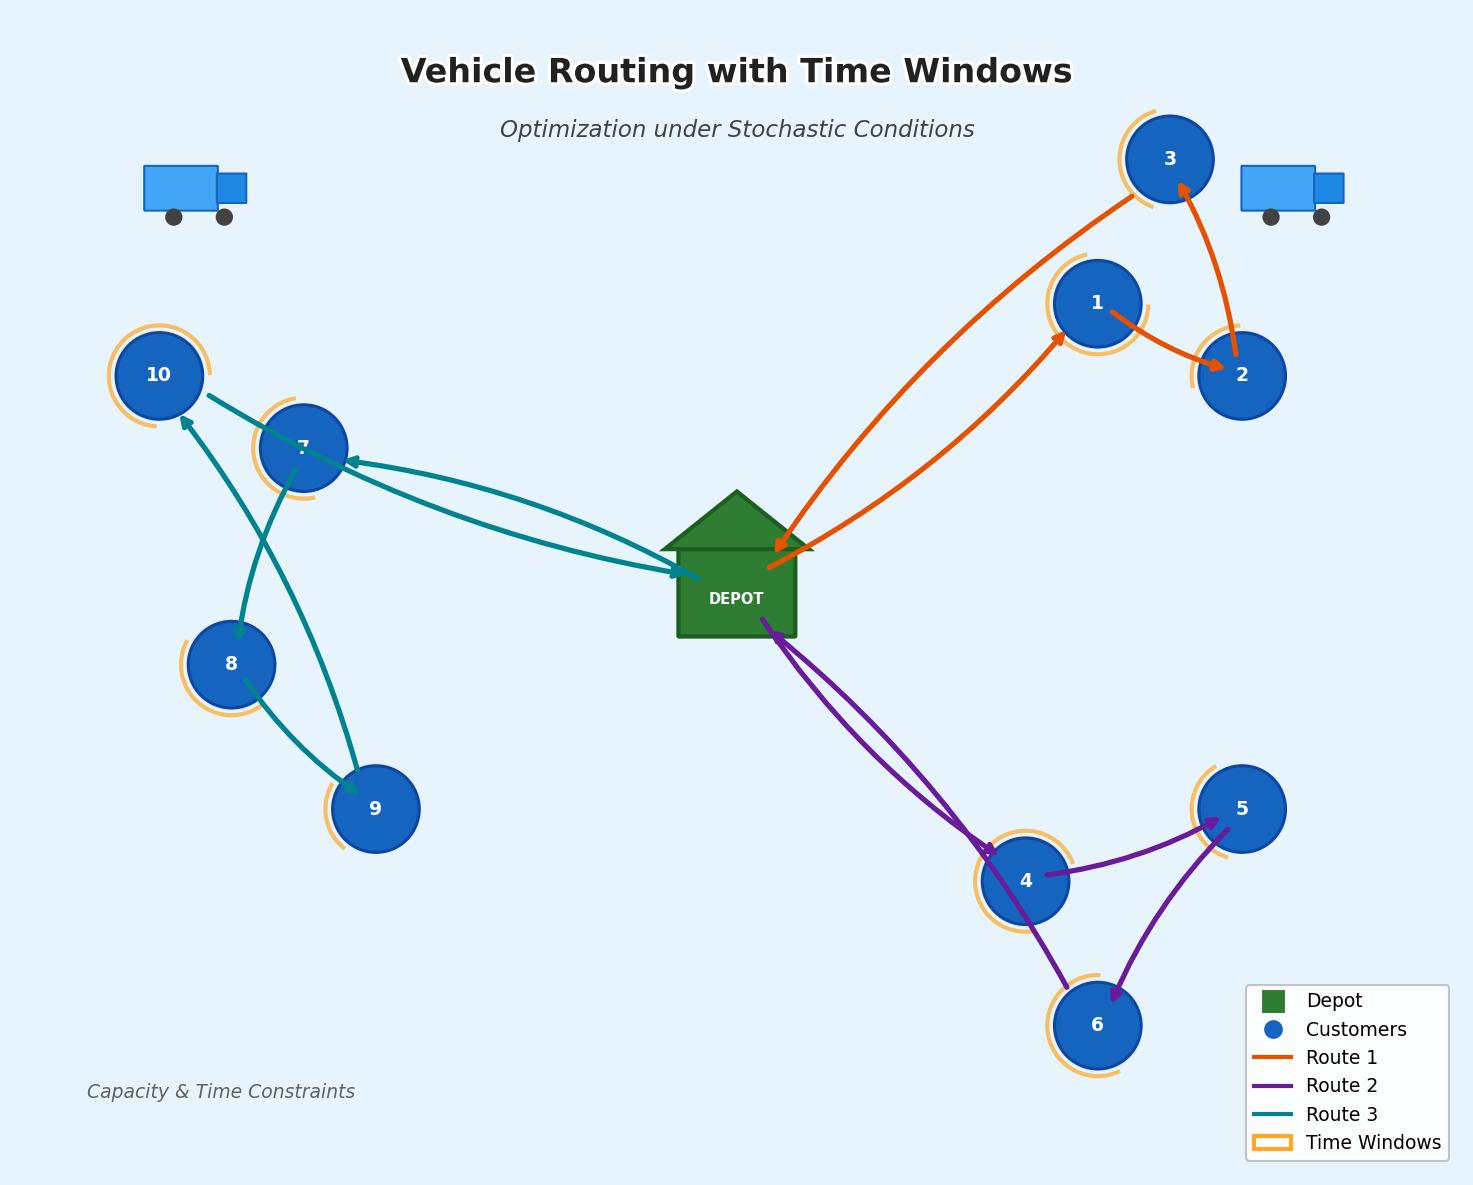
\includegraphics[width=0.7\linewidth]{img/vrp_optimization_illustration.jpg} 
	\end{center}
	\caption{Conceptual illustration of flexible delivery scheduling challenges and algorithmic optimization comparison (Tabu Search vs. Greedy). Source: AI-generated graphic.} \label{fig:conceptual_illustration}
\end{figure}

\subsection{Research hypotheses}
To evaluate the effectiveness and operational robustness of the proposed approaches, we formulate the following research hypotheses:

\begin{itemize}
    \item[\textbf{H1.}] The metaheuristic (Tabu Search) provides a lower expected total cost than the greedy algorithm across stochastic scenarios. This hypothesis tests whether the intelligent search process offers better average performance when uncertainty is introduced into customer time windows and demands.
    
    \item[\textbf{H2.}] The Tabu Search exhibits smaller variability of results across scenarios. This indicates higher operational robustness, as the solution quality remains more stable when faced with changes in input data.
    
    \item[\textbf{H3.}] The Tabu Search minimizes the total penalty associated with time-window violations compared to the greedy approach. While zero penalty may not always be achievable due to infeasible configurations of windows, the goal is to reduce the overall magnitude of violations.
    
    \item[\textbf{H4.}] The Tabu Search reduces the loss tail — that is, the occurrence and severity of extreme-cost scenarios. By lowering the frequency and impact of high-cost outliers, the algorithm provides more reliable performance in worst-case conditions.
    
\end{itemize}

The above hypotheses focus not only on average performance but also on the stability and reliability of solutions in uncertain conditions. This allows the analysis to move beyond nominal optimization and assess the algorithms’ behavior in the presence of stochastic disturbances — a crucial factor in real-world logistics operations.

% \textbf{Tutaj trzeba jeszcze trochę dopisać o motywacji }

% FIGURE 
% An example of a floating figure using the graphicx package.
% Note that \label must occur AFTER (or within) \caption.
% For figures, \caption should occur after the \includegraphics.
% Note that IEEEtran v1.7 and later has special internal code that
% is designed to preserve the operation of \label within \caption
% even when the captionsoff option is in effect. However, because
% of issues like this, it may be the safest practice to put all your
% \label just after \caption rather than within \caption{}.
%
% Reminder: the "draftcls" or "draftclsnofoot", not "draft", class
% option should be used if it is desired that the figures are to be
% displayed while in draft mode.
%
%\begin{figure}[!t]
%\centering
%\includegraphics[width=2.5in]{myfigure}
% where an .eps filename suffix will be assumed under latex,
% and a .pdf suffix will be assumed for pdflatex; or what has been declared
% via \DeclareGraphicsExtensions.
%\caption{Simulation Results}
%\label{fig_sim}
%\end{figure}

% Note that IEEE typically puts floats only at the top, even when this
% results in a large percentage of a column being occupied by floats.


% An example of a double column floating figure using two subfigures.
% (The subfig.sty package must be loaded for this to work.)
% The subfigure \label commands are set within each subfloat command, the
% \label for the overall figure must come after \caption.
% \hfil must be used as a separator to get equal spacing.
% The subfigure.sty package works much the same way, except \subfigure is
% used instead of \subfloat.
%
%\begin{figure*}[!t]
%\centerline{\subfloat[Case I]\includegraphics[width=2.5in]{subfigcase1}%
%\label{fig_first_case}}
%\hfil
%\subfloat[Case II]{\includegraphics[width=2.5in]{subfigcase2}%
%\label{fig_second_case}}}
%\caption{Simulation results}
%\label{fig_sim}
%\end{figure*}
%
% Note that often IEEE papers with subfigures do not employ subfigure
% captions (using the optional argument to \subfloat), but instead will
% reference/describe all of them (a), (b), etc., within the main caption.



